\begin{equation}
\frac{d^3\sigma}{dx_1dx_2d\cos{\hat{\theta}}} = f_\gamma^{p}(x_1,-\hat{t}) f_\gamma^{Pb}(x_2) \frac{\pi\alpha^2}{\hat{s}} \frac{\hat{t}}{\hat{u}}
+ f_\gamma^{p}(x_1,-\hat{u}) f_\gamma^{Pb}(x_2) \frac{\pi\alpha^2}{\hat{s}} \frac{\hat{u}}{\hat{t}},
\nonumber
\end{equation}

\begin{equation}
\hat{t} = -\frac{\hat{s}}{2}\left(1-\cos{\hat{\theta}}\right),
\nonumber
\end{equation}

\begin{equation}
\hat{u} = -\frac{\hat{s}}{2}\left(1+\cos{\hat{\theta}}\right),
\nonumber
\end{equation}

\begin{equation}
f_\gamma^{Pb}(x) = \frac{2Z_{Pb}^2\alpha}{\pi x}
\left(
\frac{x}{x_0}K_0(x/x_0)K_1(x/x_0)-\frac{1}{2}\frac{x^2}{x_0^2}
     \left(
      K_1^2(x/x_0)-K_0^2(x/x_0)
     \right)
\right),
\nonumber
\end{equation}

\begin{equation}
x_0 = \frac{1}{b_{min}A_{Pb}m_p},
\nonumber
\end{equation}

\begin{equation}
b_{min} = 1.1A_{Pb}^{\frac{1}{3}} \cdot 5.068 GeV^{-1}.
\nonumber
\end{equation}


Different approximations for equivalent photon flux from proton  [Phys.Rev. C87 (2013) no.2, 028201]:

1. Minimum impact parameter $b_{min} = 0.7fm$:

\begin{equation}
f_\gamma^{p}(x) = \frac{2\alpha}{\pi x}
\left(
\xi K_0(\xi)K_1(\xi)-\frac{1}{2}\xi^2
     \left(
      K_1^2(\xi)-K_0^2(\xi)
     \right)
\right),
\nonumber
\end{equation}

\begin{equation}
\xi = x m_p b_{min}, \quad b_{min} = 0.7 \cdot 5.068 GeV^{-1}.
\nonumber
\end{equation}

2. Electric:

\begin{equation}
f_\gamma^{p}(x) = \frac{\alpha}{\pi}
\left(
\frac{1-x+0.5x^2}{x}
\right)
\left(
\frac{A+3}{A-1}\log{A}-\frac{17}{6}-\frac{4}{3A}+\frac{1}{6A^2}
\right),
\nonumber
\end{equation}

\begin{equation}
A = 1+\frac{0.71 GeV^2(1-x)}{x m_p^2}.
\nonumber
\end{equation}

3. Drell and Zeppenfeld:

\begin{equation}
f_\gamma^{p}(x) = \frac{\alpha}{\pi}
\left(
\frac{1-x+0.5x^2}{x}
\right)
\left(
\log{A}-\frac{11}{6}+\frac{3}{A}-\frac{3}{2A^2}+\frac{1}{3A^3}
\right).
\nonumber
\end{equation}

\begin{table}[!ht]
\begin{center}
\begin{tabular}{|l|l|l|}
\hline
Contribution & $p_T(\ell) > 4$ GeV & $p_T(\ell) > 4$ GeV, $|\eta(\ell)| < 2.4$,\\
& & $M(\ell^+\ell^-) > 10$ GeV\\
\hline
$\gamma_{el}\gamma_{el}$ [$b_{min}=0.7fm$] & 47.4(2) nb & 18.0(1) nb\\
\hline
$\gamma_{el}\gamma_{el}$ [Electric] & 46.8(1) nb & 18.2(1) nb\\
\hline
$\gamma_{el}\gamma_{el}$ [DZ] & 55.5(1) nb & 20.2(1) nb\\
\hline
CT14qed\_proton ($\gamma_{el}$)& 52.8(1) nb & 23.1(1) nb\\
\hline
CT14qed\_inc\_proton ($\gamma_{inc}$)& 103.2(1) nb & 41.8(1) nb\\
\hline
LUXqed17\_plus\_PDF4LHC15\_nnlo\_100 ($\gamma_{inc}$)& 111.4(1) nb & 46.4(1) nb\\
\hline
NNPDF31\_nlo\_as\_0118\_luxqed ($\gamma_{inc}$) & 121.7(1) nb & 48.3(1) nb\\
\hline
MRST2004qed\_proton ($\gamma_{inc}$) & 119.1(1) nb & 41.7(1) nb\\
\hline
\end{tabular}
\end{center}
\end{table}

\clearpage

\begin{figure}
\begin{center}
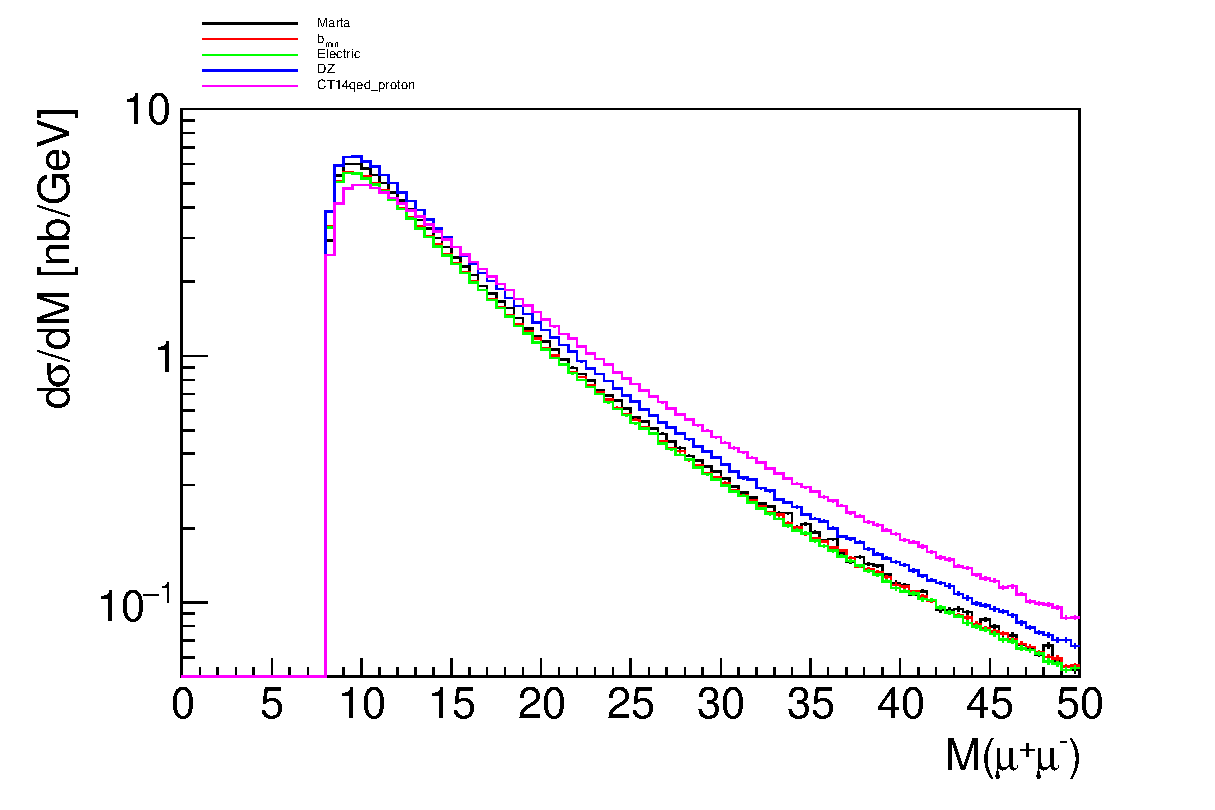
\includegraphics[width = 0.45\textwidth]{figures/M.eps}
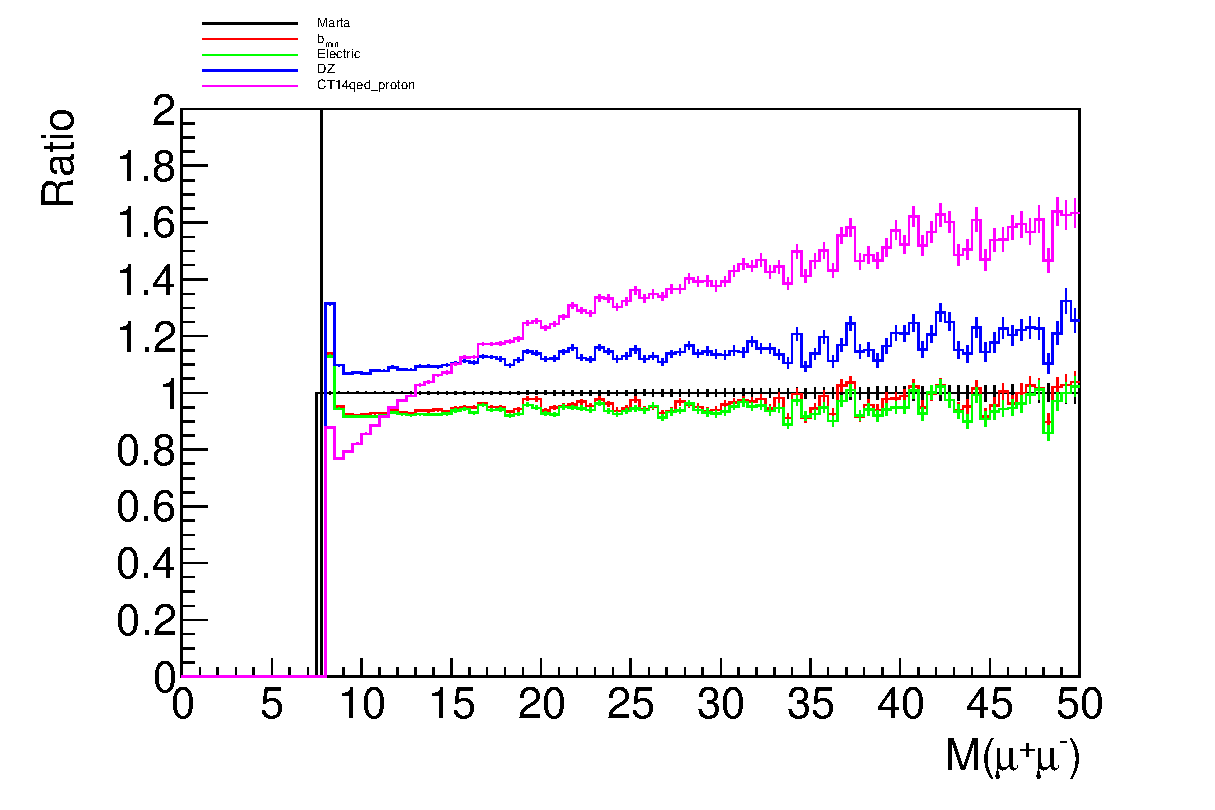
\includegraphics[width = 0.45\textwidth]{figures/RatioM.eps}
\end{center}
\caption {Distribution on $M(\mu^+\mu^-)$.}
\label{fig1}
\end{figure}

\begin{figure}
\begin{center}
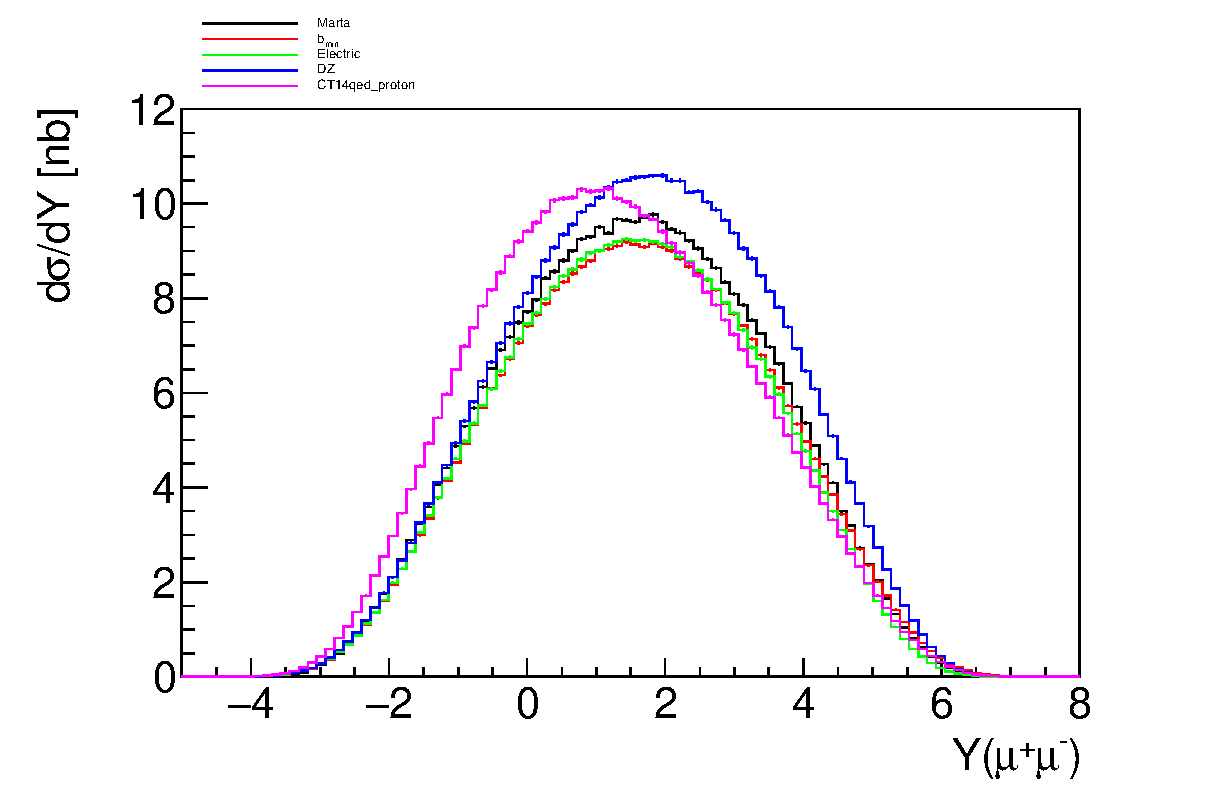
\includegraphics[width = 0.45\textwidth]{figures/Y.eps}
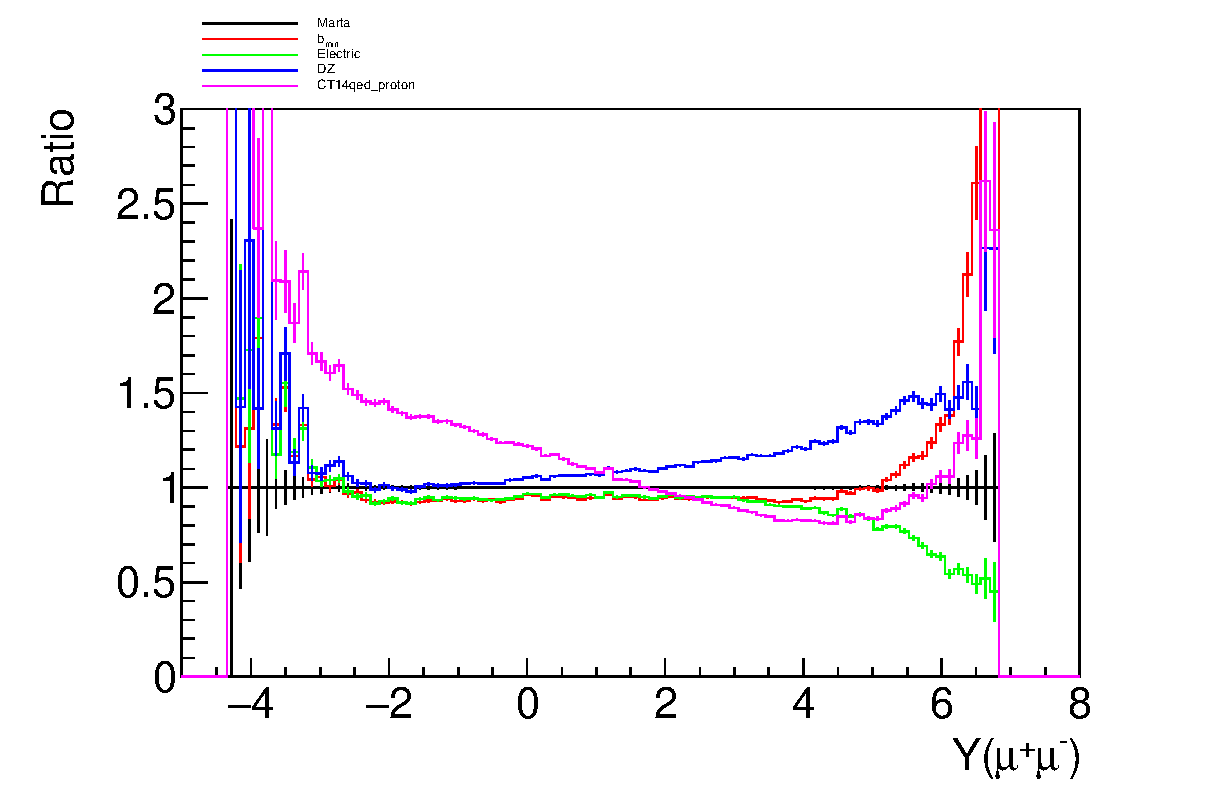
\includegraphics[width = 0.45\textwidth]{figures/RatioY.eps}
\end{center}
\caption {Distribution on $Y(\mu^+\mu^-)$.}
\label{fig2}
\end{figure}

